% ****** Start of file apssamp.tex ******
%
%   This file is part of the APS files in the REVTeX 4.1 distribution.
%   Version 4.1r of REVTeX, August 2010
%
%   Copyright (c) 2009, 2010 The American Physical Society.
%
%   See the REVTeX 4 README file for restrictions and more information.
%
% TeX'ing this file requires that you have AMS-LaTeX 2.0 installed
% as well as the rest of the prerequisites for REVTeX 4.1
%
% See the REVTeX 4 README file
% It also requires running BibTeX. The commands are as follows:
%
%  1)  latex aps25samp.tex
%  2)  bibtex apssamp
%  3)  latex apssamp.tex
%  4)  latex apssamp.tex
%
\documentclass[%
 reprint,
nofootinbib,
%superscriptaddress,
%groupedaddress,
%unsortedaddress,
%runinaddress,
%frontmatterverbose,
%preprint,
%showpacs,preprintnumbers,
%nofootinbib,
%nobibnotes,
%bibnotes,
aps,
%pra,
%prb,
%rmp,
%prstab,
%prstper,
%floatfix,
]{revtex4-1}



\usepackage[utf8]{inputenc}
\usepackage[english]{babel}
\usepackage{dsfont}
\usepackage{amsmath}
\usepackage{ mathrsfs }
\usepackage{amssymb}
\usepackage{graphicx}% Include figure files
\usepackage{dcolumn}% Align table columns on decimal point
\usepackage{bm}% bold math
\usepackage{amsmath}
\usepackage{varioref}
\usepackage{booktabs}
\usepackage[bottom]{footmisc}
\usepackage{minted} % for pseudocode

\usepackage{physics}
\usepackage[ruled,vlined]{algorithm2e}
\usepackage{algpseudocode}
\usepackage{listings}

\usepackage{booktabs}

\usepackage{tikz}
\usepackage{float}
\usepackage{siunitx}



\newcolumntype{C}{>{$}c<{$}}
\AtBeginDocument{
\heavyrulewidth=.08em
\lightrulewidth=.05em
\cmidrulewidth=.03em
\belowrulesep=.65ex
\belowbottomsep=0pt
\aboverulesep=.4ex
\abovetopsep=0pt
\cmidrulesep=\doublerulesep
\cmidrulekern=.5em
\defaultaddspace=.5em
}

\usepackage{ntheorem}
\newtheorem{theorem}{Teorem}
\newtheorem*{theorem-non}{Teorem}
\usepackage{hyperref}% add hypertext capabilities
%\usepackage[mathlines]{lineno}% Enable numbering of text and display math
%\linenumbers\relax % Commence numbering lines

%\usepackage[showframe,%Uncomment any one of the following lines to test
%%scale=0.7, marginratio={1:1, 2:3}, ignoreall,% default settings
%%text={7in,10in},centering,
%%margin=1.5in,
%%total={6.5in,8.75in}, top=1.2in, left=0.9in, includefoot,
%%height=10in,a5paper,hmargin={3cm,0.8in},
%]{geometry}

% \renewcommand{\vec}[1]{\mathbf{#1}} %ny definisjon av \vec så det blir bold face i stedet for vector-pil.

\begin{document}


\title{En videnskablig analyse af den maritime tommelfingerregel for vurderingen af kollisionskurs ved betragtning af baggrundens relative bevægelse til et andet fartøj}
\author{Mikkel Metzsch Jensen}

\affiliation{Department of Physics, University of Oslo\\}
\date{\today}


\begin{abstract}
  In this article we investegate the rule of thumb for recognizing when two boats are on a collision course. The proposed statement to be analyzed, namely \textit{The background method}, can be formulated briefly as: "If the static background seen behind the oncoming boat does not visually move relatively to the boat, then you are on a collision course.". The analysis have shown that this statement is strongly related to the dertermination of the relative bearing. By mathematical proof we found that if and only if two boats with constant velocity which approaches each other in distance have constant relative bearing they are on collision couse. Therefore the determination of the relative bearing is the most precise way of recognizing a collision course. On the other hand we found that the background method can be used as a means to determine whether the relative bearing is constant in special cases. This were mainly derived by an analytical approach but is also supported by numerical simmulations. In general the background method is found to be valid when used in greater distances to the coast, losely estimated to approximately 800 meters or more (safe distance to use). The exact estimat builds on the velocity of the observer and the tolerance definition for a humanly recognizable angular velcoty and is dependent on the value of the relative bearning and the angle between the heading and the coast. The nature of this relationship is showcased on figure \ref{fig:limit_dimension} and \ref{fig:limit_coastdis}.
\end{abstract}


\maketitle



\section{Introduktion}
Som søfarer findes der en række nødvendige og basale regler som sikrer god orden og sikkerhed til søs. Heriblandt har vi vigereglerne som regulerer færdslen på vandet og forebygger, at skibe støder sammen \cite{respektforvand}. Disse regler beskriver som udgangspunkt hvordan man skal agere hvis man er på kollisionskurs med andre fartøjer. Hertil er det fordelagtigt for søfaren at blive opmærksom på en mulig kollision i så god tid som mulig, så man kan korrigere kurs eller fart. \par
Denne rapport udsprigner af en diskussion med Lars Juel Hansen (sommeren 2019) om en forslået tommelfingerregel for netop vurderingen af en muilig kollisionskurs. Formuleringen for det vi fremadrettet skal kalde for \text{baggrundsmetoden} lyder som følger:
\begin{quote}
Betrakt båden med mulig kollisionskurs til og noter et fastliggnede punkt i baggrunden som synes akkurat bag båden. Hvis dette baggrundspunkt i den efterfølgende observationsperiode lader til at flytte sig i forhold til båden, da er du ikke på kollisionskurs med båden. Forbliver baggrundspunktet derimod i sigtelinjen bag båden er dette en indikator på kollisionskursen er reel.
\end{quote}
Ved en undersøgelse af tilgængelige internetkilder findes forskellige gengivelser af denne regel. Ifølge \cite{duelighed} kan man ved "betydelige afstande" til kysten bruge observationen om hvordan kollisionsfartøjet trækker "over land" til at vurdere pejlingen (Retning fra iagttageren til den genstand, der pejles \cite{ordbog}). Altså hævdes det at hvis den modsejlende trækker mod højre (styrbord) i forhold til baggrunden så vil fartøjet gå højre om iagterens fartøj. Modsat vil det gå venstre (bagbord) om iagterens fartøj hvis det trækker til venstre over land. Hvis ikke fartøjet bevæger sig kendeligt i forhold til baggrunden, vil det efter sigende, i overenstemmelse med baggrundsmetoden, indikere at fartøjerne er på kollisionskurs. Dog er det værd at bemærke at denne metode indføres som et middel til at vurdere om der er pejltræk (om pejlingen ændres). I andre kilder som \cite{studienoter}, \cite{retsinformation} og \cite{groensund}, er det netop pejlingen som angives som den direkte indikator på kollisionskurs. For at afgøre om der er pejltræk kan man se om det andet fartøj bevæger sig relativ til et fastliggende punkt på eget fartøj. Vi vil fremadrettet betegne denne metode som \textit{lokalpunktsmetoden}. \par
I denne rapport skal vi fremføre en matematisk analysere af baggrundsmetodens pålidelighed som indikator for kollisionskurs. Dette gøres ved først at beskrive pejlingens betydning for denne vurdering, og dernæst vurdere om der er sammenfald mellem de to metoder. Med dette udgangspunkt skal vi undersøge baggrundsmetodens præcision i forhold til at vurdere pejltræk og dermed udpege eventuelle begrænsninger.\par
Rapporten bestræber sig på at give en fyldestgørende beskrivelse af det omtalte problem, samtidig som at dette formidles til en målgruppe uden særlig matematisk baggrund. Dette er ikke mulig på alle punkter, da en ordenlig bevisførelse kræver en hvis mængde matematik. Jeg har dog forsøgt at gengive de underliggende resultater og vigtiste pointer undervejs, således at man kan springe beregninger og udledninger over uden at miste kontekst. Dette gælder f.eks. særlig udledningen i afsnit \ref{sec:pejling_betydning}.


\section{Metode}
\subsection{Definering af problemet}
Vi forestiller os to både til søs, som nærmer sig hinanden. Vi kalder den ene båd for hovedbåden (HB), hvor vi har placeret iagtageren, og den anden båd kalder vi for kollisionsbåden (KB). Vi antager at begge bådene bevæger sig med konstant hastighed, dvs. retlinjet og med konstant fart. Vi beskriver hver båd som et enkelt punkt i et to-dimensionsjonalt aksesystem som tilsvarer bådens position på vandets overflade. Vi bruger aksetitlerne x og y til at beskrive denne position $\vec{P} = (x, y)$ . Positionen til hver båd bliver da en funktion af tid, som er bestemt af parametrene: Startposition $\vec{P}_0$ og hastighed $\vec{v}$. For de to både har vi dermed bevægelseslingingen
\begin{align}
  \vec{P}(t) =  \vec{P}_0 + \vec{v}\cdot t
  \label{eq:motion}
\end{align}
Vi definerer en kollision som tilfællet hvor bådene har samme position til samme tidspunkt. Bemærk at en kollision i praksis vil ske i flere tilfælle da vi ikke har taget hensyn til bådenes udstrækning her. Dette regnes dog for en ubetydelig detalje, da man i praksis har at iagteren er placeret et fast sted på HB lige så vel som iagteren må vælge at pejle til et bestemt punkt på KB. \par
For at vudere om bådene er på kollisionskurs er det angiveligt nyttigt at benytte pejlingen. Vi definerer i matematisk forstand pejlingen $\theta_{HB}$ fra HB som vinklenen mellem kursen til HB og sigtelinjen fra HB til KB. Dette er illustreret på figur \ref{fig:metode_tegning}.

\begin{figure}[H]
  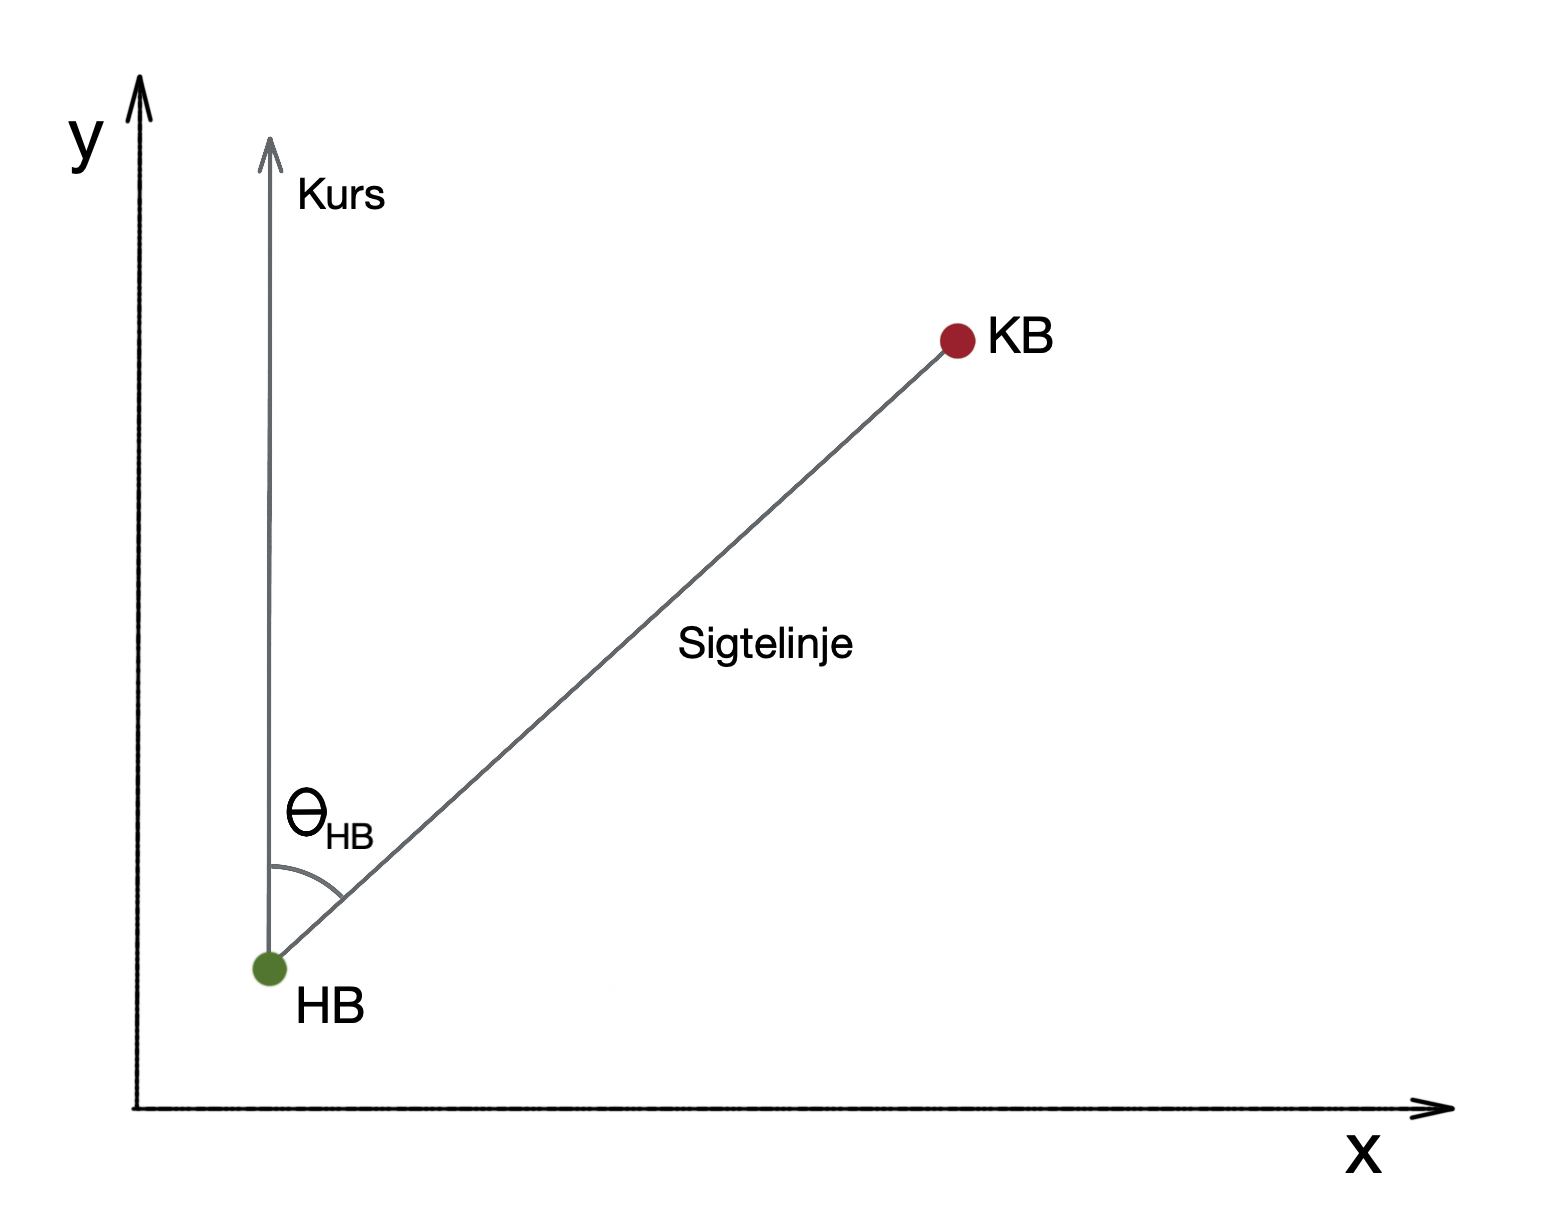
\includegraphics[width=\linewidth]{figures/metode_tegning.png}
  \caption{En illustration af pejlingen $\theta_{HB}$ som defineres som vinklen mellem kursen til HB og sigtelinjen fra HB til KB.  }
  \label{fig:metode_tegning}
\end{figure}

\subsection{Numeriske simuleringer som støtte til matematiske resultater}\label{sec:numerical_method}
I tillæg til den matematiske analyse vil vi bruge numeriske metoder som som støtte til resultaterne. Da alle bevægelserne er lineære kan vi simmulere bådenes præcise bevægelse uden usikkerhed. Dette gøres ved at evaluere bevægelsesligning \ref{eq:motion} ved forskellige tidspunkter. Dette er analogt til eulers metode uden acceleration. Vi skriver simmuleringskoden i python som angivet nedenfor. Denne er også tilgængelig på github \cite{github} sammen med diverse scripts for plotting af data.

\begin{minted}[breaklines, breakautoindent = true]{python}
import numpy as np

def simulator(MB_start, OB_start, MB_end, OB_end, T = 10, dt = 0.1):
    K = int(T/dt + 1)         #Steps
    MB_pos = np.zeros((K,2))  #MB = Main Boat
    OB_pos = np.zeros((K,2))  #OB = Other Boat
    t = np.zeros(K)           #Time

    #Initial position
    MB_pos[0] = MB_start
    OB_pos[0] = OB_start

    #Calculate constant velocity
    MB_vel = (MB_end - MB_pos[0])/T
    OB_vel = (OB_end - OB_pos[0])/T

    #Main update loop
    for k in range(K - 1):
        MB_pos[k+1] = MB_pos[k] + MB_vel*dt
        OB_pos[k+1] = OB_pos[k] + OB_vel*dt
        t[k+1] = t[k] + dt
    return MB_pos, OB_pos
\end{minted}


\section{Resultater}

\subsection{Pejlingens betydning for kollisionskurs (matematisk udledning)}\label{sec:pejling_betydning}
Da vi har antaget at bådene bevæger sig med konstant hastighed kan vi bruge en lineær transformation til at skifte koordinatsystem til intertialsystemet hvor HB er i ro (HB's intertialsystem). Med andre så kan vi frit vælge at beskrive positionen til KB som den opleves for en iagtager ombord på HB. Positionen $\vec{P}'_{KB}$ til KB i det nye intertialsystem kan skrives:
\begin{align*}
  \vec{P'}_{KB}(t) &= \vec{P}_{KB}(t) - \vec{P}_{HB}(t) \\
  &= \vec{P}_{0,KB} + \vec{v}_{KB}t - \vec{P}_{0,HB} - \vec{v}_{HB}t \\
  &= (\vec{P}_{0,KB} - \vec{P}_{0,HB}) + (\vec{v}_{KB} - \vec{v}_{HB})t \\
  &= \vec{P'}_{0,KB} + \vec{v'}_{KB}t
\end{align*}
Vi ser at $\vec{P}'_{KB}$ også beskriver en retlinjet bevægelse. I tilfællet hvor bådene er på kollisionskurs ved vi at $\vec{P}'_{KB}(t_k) = \vec{0}$ ved kollisionstidspunktet $t_{k}$. Dette medfører sammenhængen:
\begin{align}
  \vec{P'}_{0,KB} &= - \vec{v'}_{KB}t_k \nonumber \\
  \begin{pmatrix} x'_{0,KB} \\ y'_{0,KB} \end{pmatrix}\frac{1}{t_k} &=   -\begin{pmatrix} v'_{x,KB} \\ v'_{y,KB} \end{pmatrix}
  \label{eq:P=v}
\end{align}
Vi kan da finde pejlingen $\theta_{HB}$ ved at omrksive $\vec{P}'_{KB}$ til polære koordinater. Her er vi bare interesseret i vinkelkoordinat $\phi_{KB}$ som kan bestemmes som
\begin{align*}
  \phi_{KB}(t) &= \arctan{\left( \frac{y'(t)}{x'(t)}\right)} \\
  &= \arctan{\left( \frac{y'_{0,KB} + v'_{y,KB}t}{x'_{0,KB} + v'_{x,KB}t}\right)}
\end{align*}
Vi bruger da sammenghængen fra ligning \ref{eq:P=v} og finder
\begin{align*}
  \phi_{KB}(t) &= \arctan{\left( \frac{y'_{0,KB} - y'_{0,KB}\frac{t}{t_k}}{x'_{0,KB} - x'_{0,KB}\frac{t}{t_k}}\right)} \\
  &= \arctan{\left(\frac{y'_{0,KB}}{x'_{0,KB}} \frac{1 - \frac{t}{t_k}}{1 - \frac{t}{t_k}}\right)} \\
  &= \arctan{\left(\frac{y'_{0,KB}}{x'_{0,KB}}\right)} = \text{konst.} \\
\end{align*}
Fra dette ser vi at vinkelkoordinat $\phi_{KB}$ er konstant (uavhængig af tid), hvilket medfører at pejlingen også er konstant:
\begin{align*}
  \theta_{HB} &= \frac{\pi}{2} - \phi_{KB} = \text{konst.}
\end{align*}
Fra dette ræsonoment har vi altså vist at pejlingen vil være konstant i tilfællet hvor bådene er på kollisionkurs. Hvis bådene følger kollisionskursen men i modsat retning (bevæger sig væk fra hianden), kan vi indføre betingelsen $\vec{P}'_{KB}(t_i) = \vec{0}$ for et tidspunkt $t_i < 0$. Derved kan vi opstille en ligning tilsvarende \ref{eq:P=v} og derved finde at pejlingen også vil være konstant i dette tilfælle. Hvis ikke bådene er på kollisionskurs er ligning \ref{eq:P=v} ikke længere gyldig og $P'_{KB}$ kan tage hvilken som helst retlinjet bane uden om $\vec{P}'_{KB} = \vec{0}$. Det betyder at $\phi_{KB}$ og dermed også pejlingen $\theta_{KB}$ vil ændre sig som funktion af tid. Dette fører til slutningen:
\begin{theorem}
  Hvis og bare hvis to både med konstant hastighed som nærmer sig i afstand har konstant pejling til hinaden er disse på kollisionskurs.
  \label{Teo:pejling}
\end{theorem}
\subsubsection{Gengivelse af konstant-pejling-udledningen uden matematisk notation}
Siden begge bådene antages at bevæge sig med konstant fart og i en ret linje vil en iagtager på HB også se at KB bevæger sig med konstant fart og i en ret linje. I tilfællet hvor bådene er på kollisionskurs vil en iagtager på HB altså se at KB har kurs direkte mod iagteren. Dette er den eneste mulige kurs hvorpå bådene kan kollidere uden at medparterne ændrer retning eller fart. Derfor følger det at pejlingen også vil være konstant i tilfællet med kollisionskurs. Det eneste andet tidspunkt at man vil opleve at pejlingen er konstant er hvis begge bådene står stille eller bevæger sig i modsat retning af hvad der kræves for kollisionskursen.


 \subsection{Grænsebetingelser for brug af baggrundsmetoden}
 Med udgangspunkt i teorem \ref{Teo:pejling} kan vi undersøge om brugen af baggrundensmetoden er en pålidelig indikator for en fremtidig kollision. Vi skal altså undersøge om det er sammenfald mellem en konstant pejling og tilfællet hvor baggrunden ikke bevæger sig relativt til sigtelinjen gennem KB. \par
 I tilfællet med kollisionskurs ved vi fra teorem \ref{Teo:pejling} at sigtelinjen fra HB gennem KB vil have en konstant vinkel. I det enkle tilfælle hvor kystlinjen er relinjet og parallel med kursen til HB vil sigtelinjens skæring med kystlinjen forflytte sig med samme hastighed som HB. Dette resultat bekræftes ved simuleringen vist på figur \ref{fig:eks1}.
 \begin{figure}[H]
   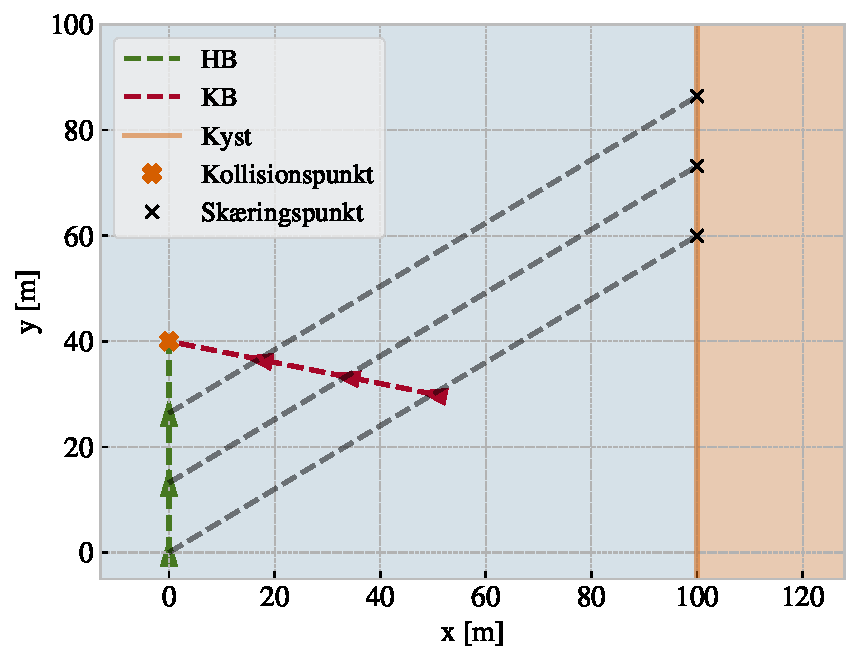
\includegraphics[width=\linewidth]{figures/eksempel1.pdf}
   \caption{En simulering af bådene HB og KB på kollisionskurs, med kollisionspunkt 100 meter fra kysten. Her plottes fire positioner for bådene (inklusiv kollisionspunktet) jævnt fordelt i tid. Fra de sorte stiblede linjer ser vi hvordan sigtelinjen fra HB gennem KB skærer med kysten. Dette skæringspunkt forflytter sig som forventet i henhold til HB's bevægelse.}
   \label{fig:eks1}
 \end{figure}
 Hvis sigtelinjens skæring med kystlinjen er kendelig, på trods af at bådene er på kollisionskurs og pejlingen er konstant, vil baggrundsmetoden være vildledene. Fra HB's perspektiv vil baggrundspunktet (BP) bevæge sig med en hastighed $\vec{v'}_{BP} = - \vec{v}_{HB}$. Dette giver en observeret vinkelhastighed $\omega_O$:
 \begin{align*}
   \omega_O = -\frac{v_{HB}\sin{(\theta_{HB})}}{d}
 \end{align*}
 hvor $v_{HB} = |\vec{v}_{HB}|$ er bådens fart, $\theta_{HB}$ er pejlingen og $d$ er afstanden til kysten via sigtelinjen. Hvis vi definerer minimumsgrænsen for en kendelig forflytning som vinkelhastigheden $\omega_k$ får vi at kriteriet for anvendelse af baggrundsmetoden er
 \begin{align}
   |\omega_O| &< \omega_k \nonumber \\
   \frac{v_{HB}\sin{(\theta_{HB})}}{d} &< \omega_k \nonumber \\
   \frac{v_{HB}\sin{(\theta_{HB})}}{\omega_k} &< d
   \label{eq:limit}
 \end{align}
Vi kan da bruge denne sammenhæng til at finde den minimume afstand $d$ for brug af baggrundsmetoden som funktion af $\theta_{HB}$. Dette resultat er vist på figur \ref{fig:limit_dimensionless}.
 \begin{figure}[H]
   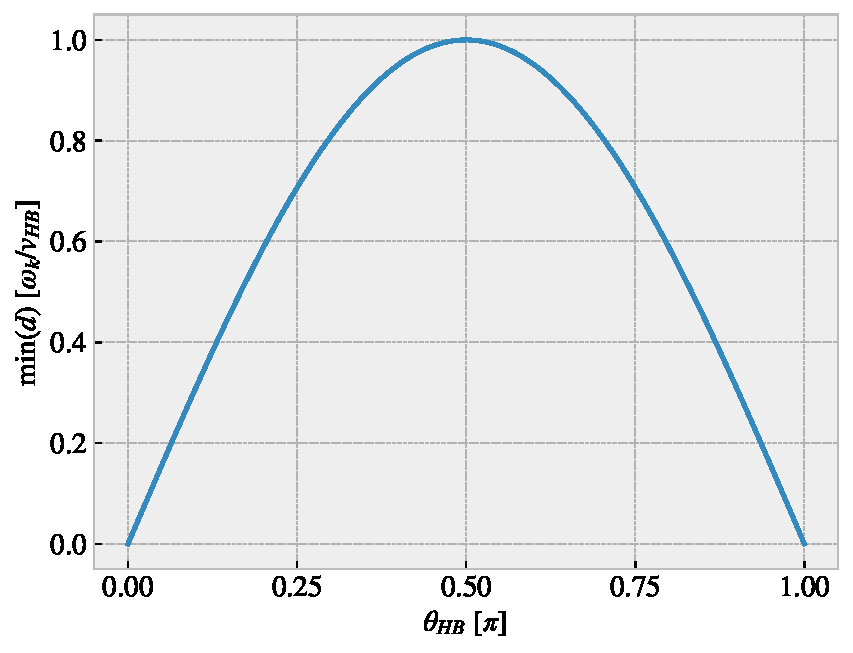
\includegraphics[width=\linewidth]{figures/limit_dimensionless.pdf}
   \caption{Den minimume afstand $\min{(d)}$ som funktion af pejlingen $\theta_{HB}$ som mulliggør brug af baggrundsmetoden. $d$ beskriver afstanden til kysten via sigtelinjen. Resultatet er angivet med dimensionløse enheder med skaleringsfaktorene $\omega_k$ som er den minimumme vinkelhastighed for en kendelig forflytning og $v_{HB}$ som er farten til HB. For at baggrundsmetoden skal være anvendelig, må vi kræve at $d$ ligger over kurven for $\min{(d)}$.}
   \label{fig:limit_dimensionless}
 \end{figure}


\subsubsection{Definering af kendelig forflyting}
For at bestemme enhederne til figur \ref{fig:limit_dimensionless}, må vi definere hvad en kendelig forflytning er. Hertil bruger vi en række kvalificerede gæt for at finde et estimat for $\omega_k$. Bemærk at følgende resultater derfor bygger på en del usikkerheder. \par
Vi kan forestille os at vi ved observation af KB vil benytte et centralt punkt på båden som referanse mod baggrunden. En mulig defintion på en kendelig forflytning kan da være at baggrundspunktet har flyttet sig ud til eller forbi kanten af båden i løbet af en observationsperiode. Observationsperioden estimeres til 10 sekunder, svarende til den nedre grænse af tidsintervallet 10-20 sekunder som nævnes i \cite{duelighed}. Vi siger da at forflytningen er kendelig hvis baggrundspunktet har flyttet sig en relativ afstand større eller lig halvdelen af bådens tværlængde set fra iagtageren i løbet af de 10 sekunder. For sejlbåde i den lidt større klasse kan vi bruge en gennomsnitlig bredde på 5 m og længde på 15 m, hvilket giver 10 m som middelestimat (tilsvarer 45 graders sigtelinje). Til sidst må vi vurdere den aftsand hvorved en søfarer har brug for at vurdere kollisionsrisikoen. Hertil bruges 200 meter som en minimumsværdi. Ud fra dette finder vi at en kendelig forflytning kan defineres ved en vinkelhastighed større eller lig $\omega_k$:
\begin{align}
  \omega_k = \frac{\arctan{(\frac{1}{2}\frac{10 \text{m}}{200 \text{m}})}}{10 \text{s}} = 0.0025 s^{-1} \approx  0.14^{\circ}s^{-1}
  \label{eq:omega_k}
\end{align}
Bemærk at disse antagelser udelukkende gøres for estimere menneskets evne til at kende en forflytning i praksis. Ved valg af den nedre grænse for observationsperioden, et stort estimat for bådens tværlængde og et minimumsestimat for afstanden mellem bådene ved observation, estimeres den øvre grænse for en kendelig forflytning. Dette vil føre til at estimatet for den gyldige afstand $d$ bliver et minimumsestimat og dermed giver de bedst tænkelige vilkår for baggrundsmetodens gyldighed. \par
Vi kan nu bruge at en typisk bådhastighed er 4 knob hvilket tilsvarer omtrent 2 m/s. Med disse værdier kan vi skalere resultatet fra figur \ref{fig:limit_dimensionless} sådan at vi får det nye resultat på figur \ref{fig:limit_dimension}
\begin{figure}[H]
  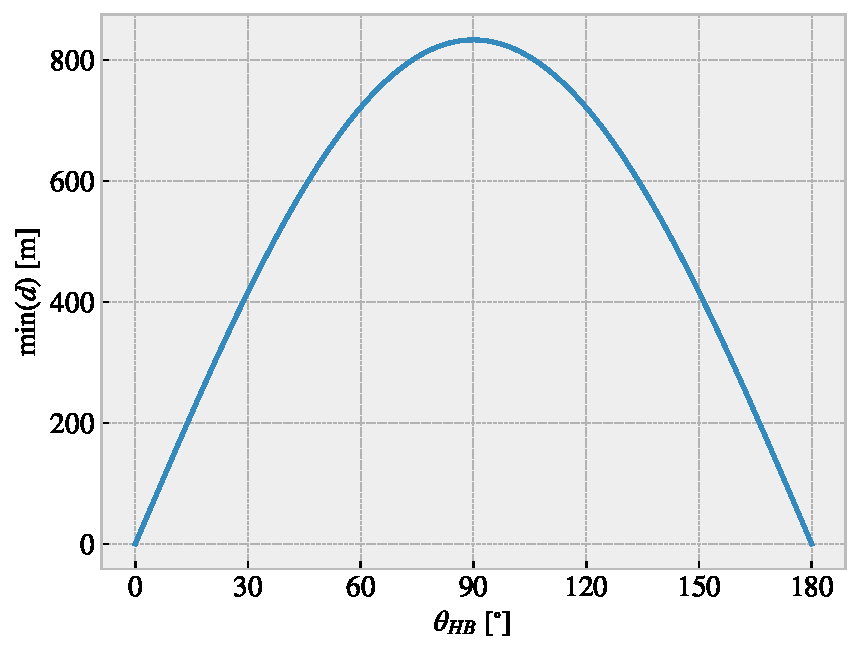
\includegraphics[width=\linewidth]{figures/limit_dimension.pdf}
  \caption{Den minimume afstand $\min{(d)}$ som funktion af pejlingen $\theta_{HB}$ som mulliggør brug af baggrundsmetoden. $d$ beskriver afstanden til kysten via sigtelinjen i meter. Enhederne er fastlagt ud fra figur \ref{fig:limit_dimension} med brug af løse estimater for $\omega_k$ og $v_{HB}$.}
  \label{fig:limit_dimension}
\end{figure}
I en situation hvor den retlinjede kyst har en vinkel $\beta$ i forhold til HB's kurs kan vi omregne afstanden $d$ langs sigtelinjen til den korteste afstand $s_{kyst}$ mellem HB og kysten (linjen vinkelretpå kysten). Omregning gøres som
\begin{align}
  s = d\cdot \sin{(\theta_{HB} + \beta)}
  \label{eq:s_kyst}
\end{align}
Ved at anvende denne omregning får vi resultatet vist på figur \ref{fig:limit_coastdis}.
\begin{figure}[H]
  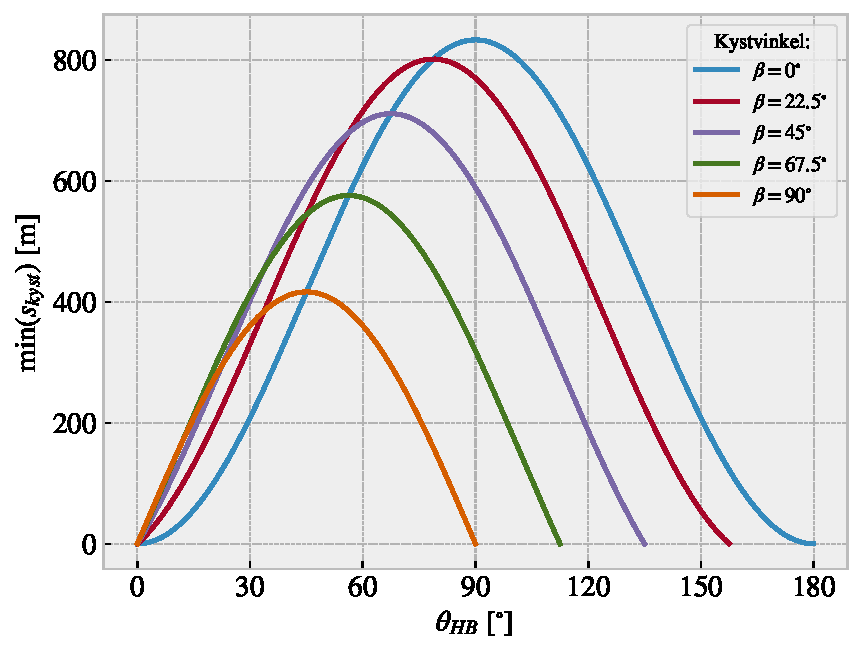
\includegraphics[width=\linewidth]{figures/limit_coastdis.pdf}
  \caption{Den minimumme afstand $\min{(s_{kyst})}$ som funktion af pejlingen $\theta_{HB}$ som mulliggør brug af baggrundsmetoden. $s_{kyst}$ (se ligning \ref{eq:s_kyst}) er den korteste afstand for HB til kysten, når kysten har en vinkel $\beta$ i forhold til HB's kurs.}
  \label{fig:limit_coastdis}
\end{figure}

Da det er upraktisk at skulle vurdere vinklen til kysten $\beta$ kan vi forsimple dette resultat lidt. Vi ser på \ref{fig:limit_coastdis} at når $\beta$ øger fra 0 til 90$^{\circ}$ så forskydes den grunnlæggende kurve for $\beta = 0$ samtidig som at den formindskes. Vi er nu intterresert i at finde en kurve som indeholder alle disse forskydninger fra variation af $\beta$, således at vi har en effektiv maksimumskurve for $\min{(s_{kyst})}$. Dette tilsvarer at vi tager den maksimale værdi for $\min{(s_{kyst})}$ i hvert punkt ved at vælge den kystvinkel $\beta$ som giver den største værdi. Vi husker på at
\begin{align*}
  s_{kyst} \propto \sin{(\theta_{HB} + \beta)}
\end{align*}
og derved ser vi, at vi opnår maksimalværdi ved at vælge $\beta = \frac{\pi}{2} - \theta_{HB}$. Da finder vi at den maksimale værdi som funktion af $\theta_{HB}$ er
\begin{align}
  \max{(s_{kyst})}(\theta_{HB}) = d
  \label{eq:max_s_kyst}
\end{align}
Bruger vi denne approksimation får vi et anvendelig plot for aflæsning af den gyldige zone for baggrundsmetoden uavhængig af kystvinklen. Dette er vist på figur \ref{fig:limit_coastdis_betamax}.
\begin{figure}[H]
  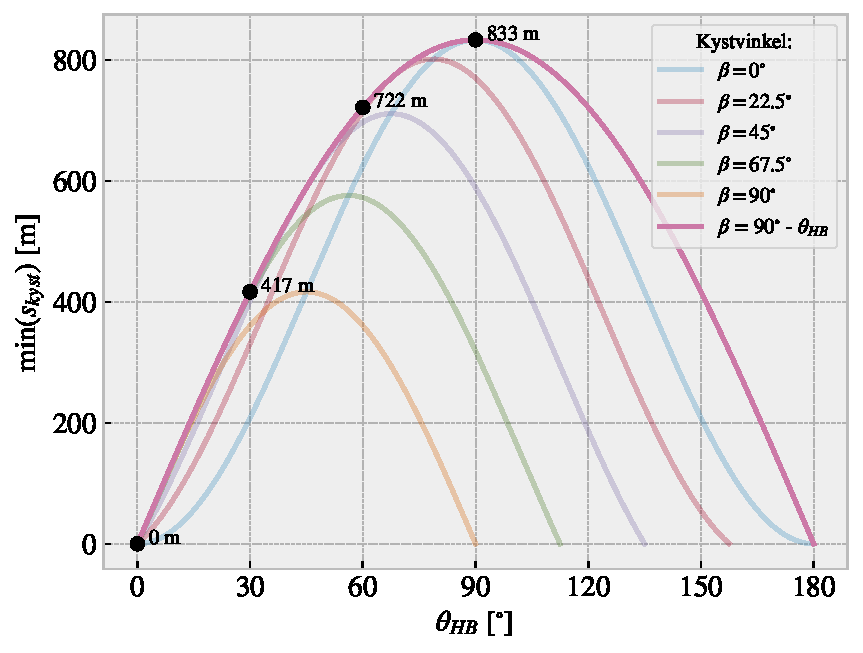
\includegraphics[width=\linewidth]{figures/limit_coastdis_betamax.pdf}
  \caption{Den minimumme afstand $\min{(s_{kyst})}$ som funktion af pejlingen $\theta_{HB}$ som mulliggør brug af baggrundsmetoden (se figur \ref{fig:limit_coastdis}). Den lyserøde kurve for $\beta = 90^{\circ} - \theta_{HB}$, tilsvarerer det valg af $\beta$ for hvert punkt som giver den største værdi. Dermed har vi et maksimumsestimat på $\min{(s_{kyst})}$ som kan aflæses uavhængig af kystvinkel $\beta$ }
  \label{fig:limit_coastdis_betamax}
\end{figure}

\subsection{Numeriske simuleringer}
Ved brug af koden vist i afsnit \ref{sec:numerical_method} har vi simmulert forskellige situationer for at understøtte de matematiske resultater. I appendix \ref{sec:appendix} findes en række plots over forskellige situationer med og uden kolliosionskurs. I tillæg findes en række animationer på github'en \cite{github}, som giver et mere intuitiv indblik i bevægelserne og hvordan pejling og baggrundspunkt ændres.


\section{Diskussion}
Ud fra den matematiske slutning om pejlingen i teorem \ref{Teo:pejling} er det klart at pejlingen kan bruges som en direkte indikator på om bådene er på kollisionskurs. Hvis KB nærmer sig og pejlingen ikke ændres er dette ensbetydene med at bådene vil kollidere, hvis ikke kurs eller retning ændres. Altså vil lokalpunktsmetoden være troværdig i alle situationer og derfor også den bedst egnede metode. \par
Som antydet i \cite{duelighed} fandt vi at baggrundsmetoden kan bruges som en indikator på om der er pejltræk eller ikke. Dette er dog ikke uden begrænsninger da baggrunden, i tilfælde med konstant pejling, vil flytte sig tilsvarende HB's relative bevægelse til baggrunden. Siden denne bevægelse bliver mindre og mindre tydelig desto længere væk fra den observerede baggrund man befinder sig, kan baggrundes metoden effektivt anvendes ved større afstande til kysten. Dette er i overenstemmelse med påstanden fra \cite{duelighed}. Med kendskab til den minimumme vinkelhastighed $\omega_k$ for en kendelig forflytning samt HB's hastighed, vil man kunne kortlægge det gyldige område for baggrundsmetoden via resultaterne fra figur \ref{fig:limit_dimensionless}. Med kvalificerede gæt på disse størrelser kom vi frem til resultatet i figur \ref{fig:limit_dimension} som giver et estimat på dette gyldige område. Bemærk dog at disse estimater er ganske usikkre og derfor kun bør tolkes som et estimat på størrelsesorden af området. \par
På figur \ref{fig:limit_coastdis} får vi relevant information om hvad afstanden $d$ tilsvarer i den direkte afstand til kysten $s_{kyst}$ som er mere anvendelig i praksis. Siden dette involverer at man som søfarer må vurdere vinklen til kysten også, kan vi hellere bruge det endelige resultat på figur \ref{fig:limit_coastdis_betamax}. Her har vi den maksimale minimumsafstand som trænges ved et vilkårlig valg af kystvinkel $\beta$. Ved aflæsning af denne figur finder vi:
\begin{table}[H]
 \begin{center}
 \caption{....}
 \begin{tabular}{|c|c|} \hline
 $\theta_{HB}$ [$^{\circ}$] & $s_{kyst}$ [m]  \\ \hline
 0 & 0 \\ \hline
 30 & 417 \\ \hline
 60 & 722  \\ \hline
 90 & 833 \\ \hline
 \end{tabular}
 \label{tab:valid_area}
 \end{center}
\end{table}
Dette giver et fornuftig billede af det gyldige område for baggrundsmetoden. Her ser vi at baggrundsmetoden kan bruges tættere på kysten når KB kommer forfra eller bagfra i en spids vinkel, mens en 90 $^{\circ}$ pejling vil være det mest krævende sted at anvende metoden.



% Altså viser det sig at kurvene på \ref{fig:limit_dimensionless} og \ref{fig:limit_dimension} kan bruges som et fornuftig estimat for $s_{kyst}$ for vilkårlige kystvinkler. Dog er enheden på disse plots misvisende for denne slutning og derfor kan vi passende indsætte figure på nyt igen her nedenfor.

% Dog ser vi på figur \ref{fig:limit_coastdis} af den største minimumsafstand $\min{(s_{kyst})}$ for hver værdi af kystvinkel $\beta$ ser ud til at have toppunkt ved skæringen med kurven for $\beta = 0$. Dette er ikke tilfældigt, da vi kan vise at dette stemmer rent matematisk. Løser vi $\frac{d s}{d \theta_{HB}} = 0$ for maksimmspunkter finder vi:
% \begin{align*}
%   &\frac{d s}{d \theta_{HB}} = \sin{(2\theta_{HB} + \beta)} = 0 \\
%   &\Longleftrightarrow \quad \theta_{max} = \frac{\pi}{2}n - \frac{\beta}{2}
% \end{align*}
% Derfra ser vi at
% \begin{align*}
%   s(\theta_{max}(x), \beta = 0) &=   d\sin{\left(\frac{\pi}{2}n - \frac{x}{2}\right)} \\
%   s(\theta_{max}(x), \beta = x) &= d\sin{\left(\frac{\pi}{2}n + \frac{x}{2}\right)}
% \end{align*}
% Her er $s(\theta_{max}(x), \beta = 0) =   s(\theta_{max}(x), \beta = x)$ lig hinandne på grund af symmetrien i sinus-funktionen. Altså kan vi retfærdiggøre at vi nøjes med at bruge den blå kurve for $\beta = 0$ på figur \ref{fig:limit_coastdis} når vi skal vurdere det gyldige område. (ELLER ER DET FAKTISK DEN BLÅ KURVE FOR d SOM KAN BRUGES SOM ET MAKSIMUM FOR ALLE BETA?) For små vinkler i området 0-30 $^{circ}$


%  mne hvis vi sammenfatter det mulige interval som funktion af pejlingen får vi datapunkterne vist på tabel \ref{tab:valid_area}.
% \begin{table}[H]
%  \begin{center}
%  \caption{....}
%  \begin{tabular}{|c|c|} \hline
%  $\theta_{HB}$ [$^{\circ}$] & $s_{kyst}$-interval [m]  \\ \hline
%  30 & [208, 402] \\ \hline
%  60 & [361, 725]  \\ \hline
%  90 & [0, 833] \\ \hline
%  \end{tabular}
%  \label{tab:valid_area}
%  \end{center}
% \end{table}
% Dette giver et bedre billede af den minimumme direkte aftsand til kysten som kræves for at baggrundsmetoden kan anvendes. \\
% \\










% Noter:\\
% \\
% Bemærk at vi i praksis må tage hensyn til at båden har en hvis udstrækning og at den dermed også kolliderer når punkterne passerer tæt forbi hinanden. Dette har dog ikke betydning for den teortiske model, og ved andvendelse af modellen i praksis må man bruge resultaterne i overensstemmelse med en ønsket sikkerhedsradius ved forbipassering. (Se diskussion for mere info om dette.)
% \\
% Baggrundsmetoden kan sandsynligvis anvendes tættere på kysten end den estimerede grænse hvis søfaren evner at tage højde for baggrundes forflytning grundet relativ forflytning til kysten
% \\
% Bestemmelsen af $\omega_k$ er et meget løst estimat. Angiver størrelsesordenen for anvendelig område.
% \\
% Klart at en mere direkte vurdering af pejlingen er fordelagtig.
% \\
% "Pejltræk til forenden af et stort skib eller til et skib med slæb er ikke tilstrækkeligt. Der skal være pejltræk til den agterste kant i sejlretningen." \cite{groensund}.
% \\
% Se bort for strømforhold, vind og andre mærkelige ting?

\section{Konklusion}
Fra den matematiske udledning kan vi konkludere at pejlingen kan bruges som en direkte indikator på at to både er på kollisionskurs. Når to både nærmer sig, med konstant hastighed, vil pejlingen være konstant hvis disse er på kollisionskurs. Hvis pejlingen ændres er disse ikke på kollisionskurs. Vi fandt at baggrundsmetoden kan bruges som en indikator på om der er pejltræk hvis iagtageren befinder sig tilstrækkelig langt væk fra baggrunden. Dette skyldes at baggrundens forflytning kan være kendelig selvom bådene er på kollisionskurs, når iagtageren befinder sig relativt nær kysten. Her er resultatet fra figur \ref{fig:limit_dimensionless} det mest generelle angivelse af det gyldige område for brug af baggrundsmetoden. Ikke desto mindre fandt vi ved brug af en række estimater afstanden til kysten som funktion af pejling som kræves for at anvende baggrundsmetoden. Dette er vist på figur \ref{fig:limit_coastdis_betamax} og vi ser at vi ved spidse vinkler for pejlingen på omrking 30 eller 150 $^{\circ}$ kan bruge baggrundsmetoden for afstande til kysten større end 417 m. Ved en pejling på 90 $^{\circ}$ var dette krav størst på 833 m. Altså tjener dette som et øvre estimat for hvornår baggrundsmetoden kan bruges med sikkerhed generelt. Siden dette er basert på usikkre antagelser bør dette dog kun tolkes som et bud på størrelsesordnen for denne grænse som altså kan sættes til 1 km i praksis.







%  Dette kan formuleres som teoremet:
%
% \begin{theorem-non}
%   Hvis og bare hvis to både har kollisionskurs og nærmer sig i afstand vil pejlingen fra den ene båd til den anden være konstant.
% \end{theorem-non}
%
% Altså når to både nærmer sig vil disse være på kollisionskurs hvis ikke det er pejltræk og omvendt hvis der er pejltræk.


% Videre fandt vi at baggrundsmetoden, hvor man vurdere om baggrunden flytter sig relativt til den anden båd, kan bruges som en indirekte indikator på kollisionskurs. Dette skyldes at baggrundens forflytning kan være kendelig selvom bådene er på kollisionskurs, når iagtageren befinder sig relativt nær kysten. Et estimat af grænseværdien for denne kystafstand er vist på figur \ref{fig:limit_coastdis} og tabel \ref{tab:valid_area}, men vi ser at generelt at baggrundsmetoden kan bruges for kystafstande på ca. 800 m eller større.
% \\
% Baggrundspunktet bevæger sig ligesom dit eget skib inde på kysten. Så spørgsmålet er om du ville kunne se en kendelig forflytning af dit eget skib (med sinus led af $\theta_{HB}$) hvis det var placeret på baggrundspunktet.





\begin{thebibliography}{9}
  \bibitem{github} Metzsch-Jensen M. (2020), \textit{Boat myth - GitHub repository}, Available at: \url{https://github.com/mikkelme/boat_myth}

  \bibitem{respektforvand} Repspekt for vand \url{https://www.respektforvand.dk/paa-havet/laer-at-sejle/vigeregler} (sidst læst: 16/01/2021)

  \bibitem{duelighed} Duelighed.dk. Date. Edition. Skipper-kursus (slide 03-02), tilgængelig ved \url{http://www.duelighed.dk/tutorial_soevejsregler/03_02.htm} (sidst læst: 05/01/2021)

  \bibitem{ordbog} Hjemmeværnet: Maritime udtryk, tilgængelig ved \url{https://www.hjv.dk/oe/HVF122/Sider/Maritime-udtryk.aspx} (sidst læst: 05/01/2021)

  \bibitem{studienoter} Søren Toftegaard O. (2013), \textit{LystSejlads}, s. 19 (afsnit 1.4) , tilgængelig ved \url{http://studienoter.dk/Sejlads/Noter/LystSejlads.pdf} (sidst læst: 05/01/2021)

  \pagebreak
  \bibitem{retsinformation} retsinformation.dk: \textit{Bekendtgørelse om søvejsregler} 20/11/2009. Regel 7: fare for sammenstød (d) (20/11/2009), tilgængelig ved \url{https://www.retsinformation.dk/eli/lta/2009/1083} (sidst læst: 05/01/2021)

  \bibitem{groensund} Albrechten S. (2007). \textit{Sejlads for Begyndere} \url{http://www.groensund.dk/upl/website/sejlads/SejladsforBegyndere2.pdf}


\end{thebibliography}

\clearpage
\onecolumngrid
\section{Appendix}\label{sec:appendix}

\subsection{Simmuleringer med kollision}

\begin{figure}[H]
  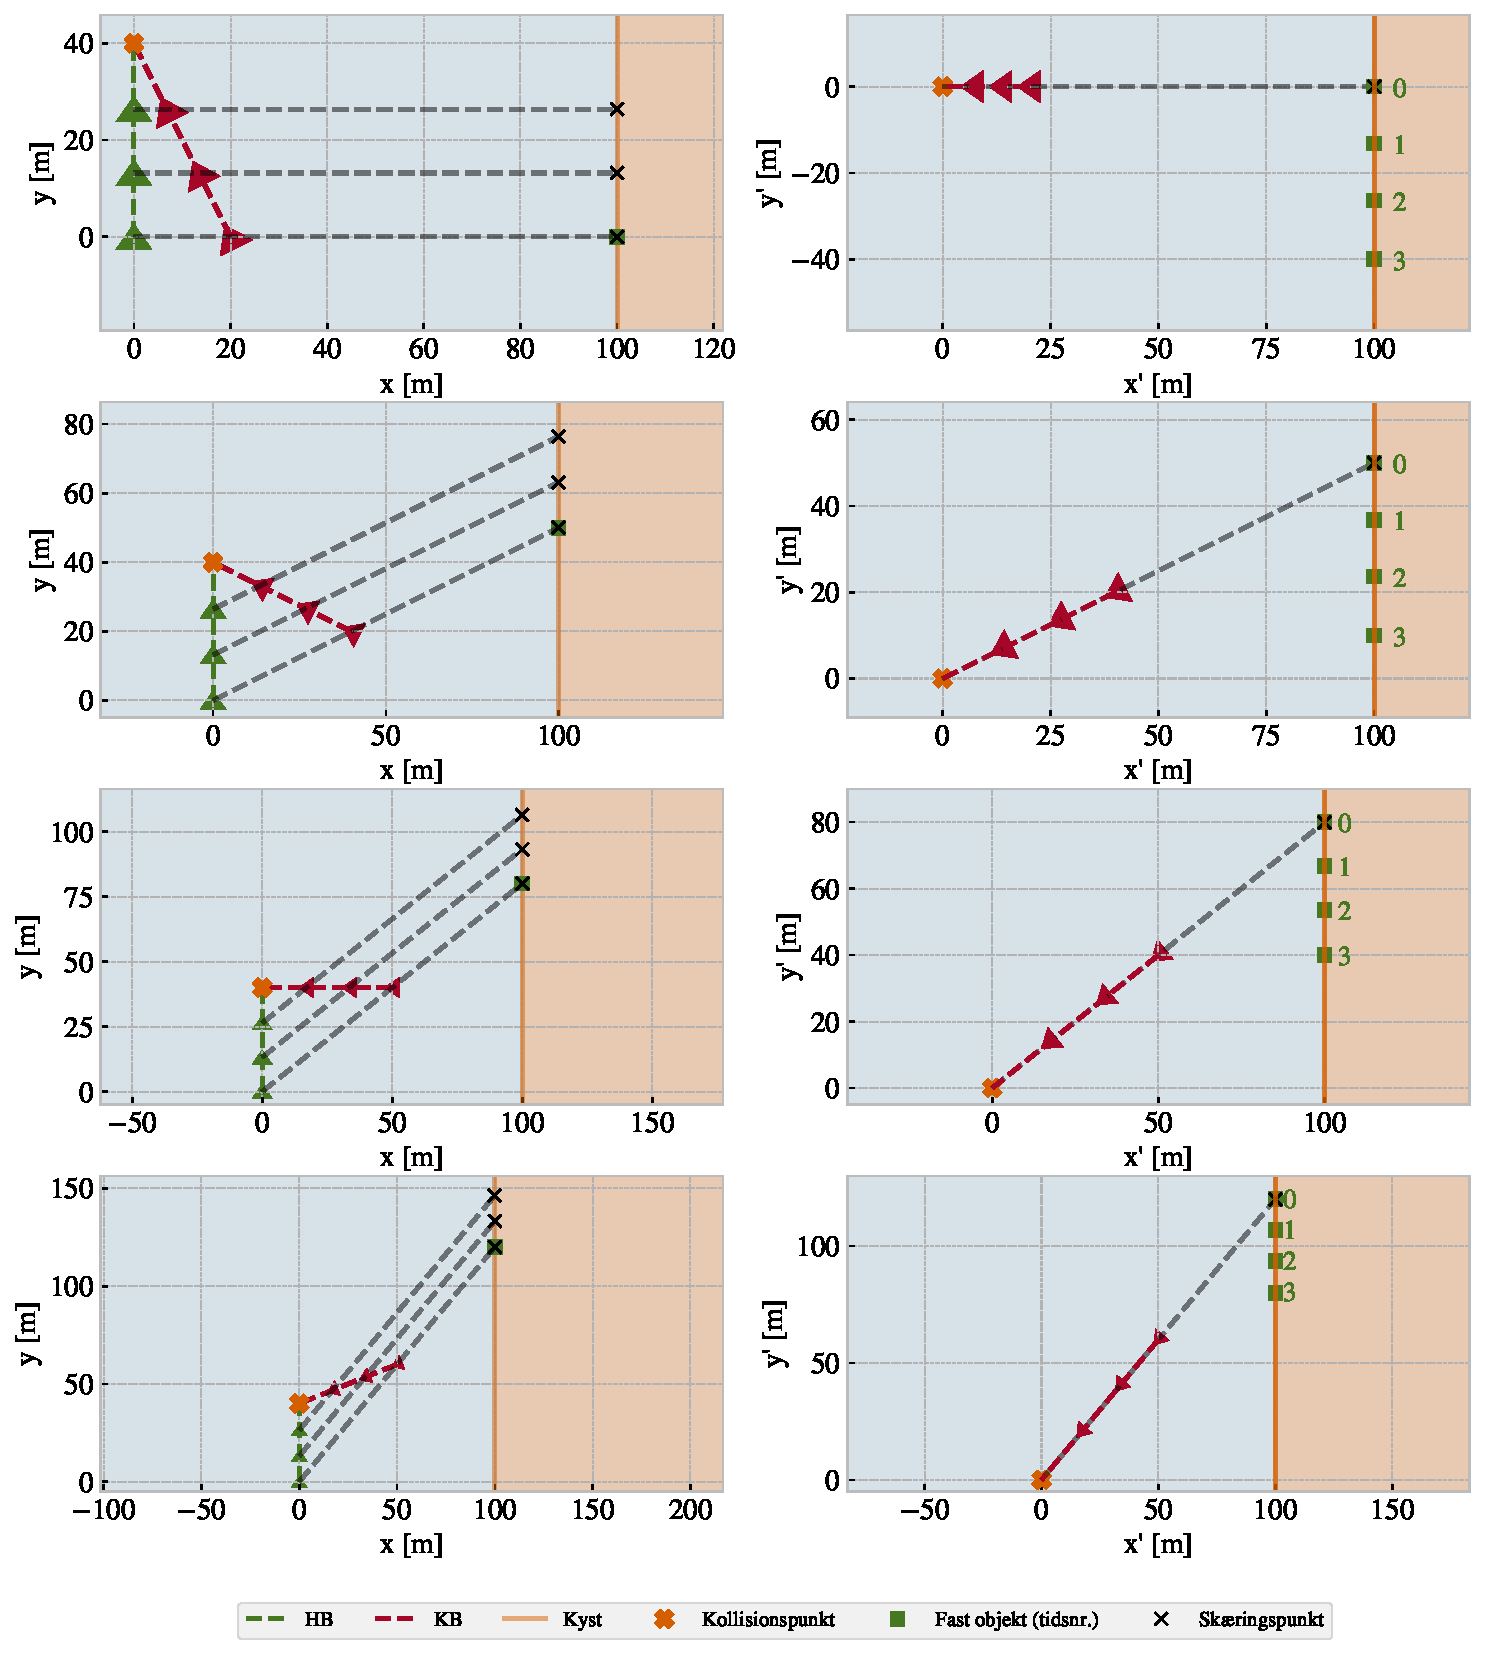
\includegraphics[width=\linewidth]{figures/subplot_C1.pdf}
  \caption[A table inside a caption]{
\begin{tabular}{|c|c|c|c|c|}
\hline
Figurrække & $HB_{start}$  & $KB_{start}$ & $HB_{slut}$ & $KB_{slut}$\\ \hline
1  & (0,0) & (20,0) & (0, 40) & (0, 40) \\ \hline
2  & (0,0) & (40,30) & (0, 40) & (0, 40) \\ \hline
3  & (0,0) & (50,40) & (0, 40) & (0, 40) \\ \hline
4  & (0,0) & (50,60) & (0, 40) & (0, 40) \\ \hline
\end{tabular}}
  \label{fig:subplot_C1}
\end{figure}

\begin{figure}[H]
  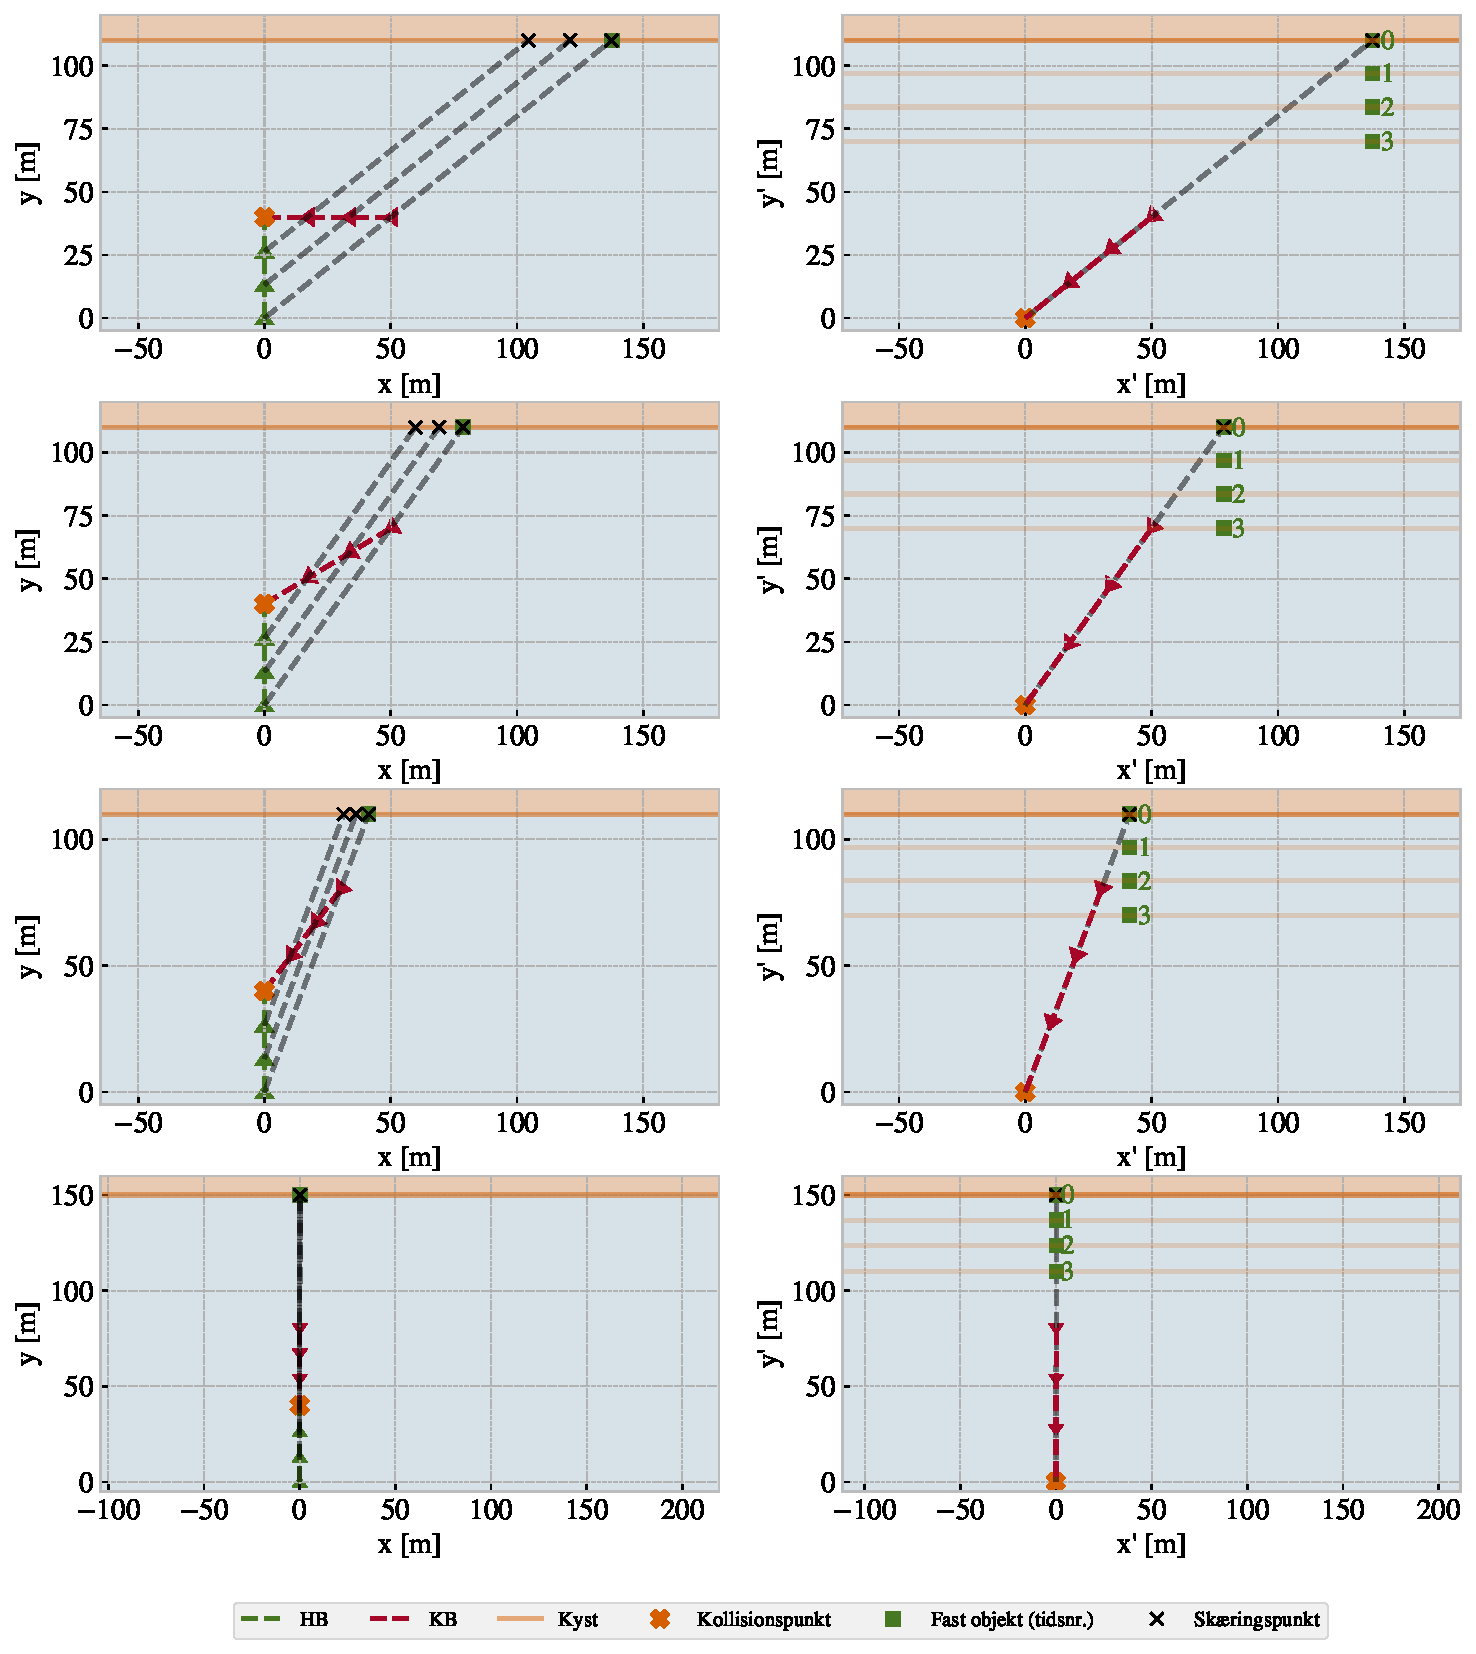
\includegraphics[width=\linewidth]{figures/subplot_C2.pdf}
  \caption[A table inside a caption]{
\begin{tabular}{|c|c|c|c|c|}
\hline
Figurrække & $HB_{start}$  & $KB_{start}$ & $HB_{slut}$ & $KB_{slut}$\\ \hline
1  & (0,0) & (50,40) & (0, 40) & (0, 40) \\ \hline
2  & (0,0) & (50,70) & (0, 40) & (0, 40) \\ \hline
3  & (0,0) & (30,80) & (0, 40) & (0, 40) \\ \hline
4  & (0,0) & (0.1,80) & (0, 40) & (0, 40) \\ \hline
\end{tabular}}
  \label{fig:subplot_C2}
\end{figure}


\clearpage
\subsection{Simmuleringer uden kollision}
\begin{figure}[H]
  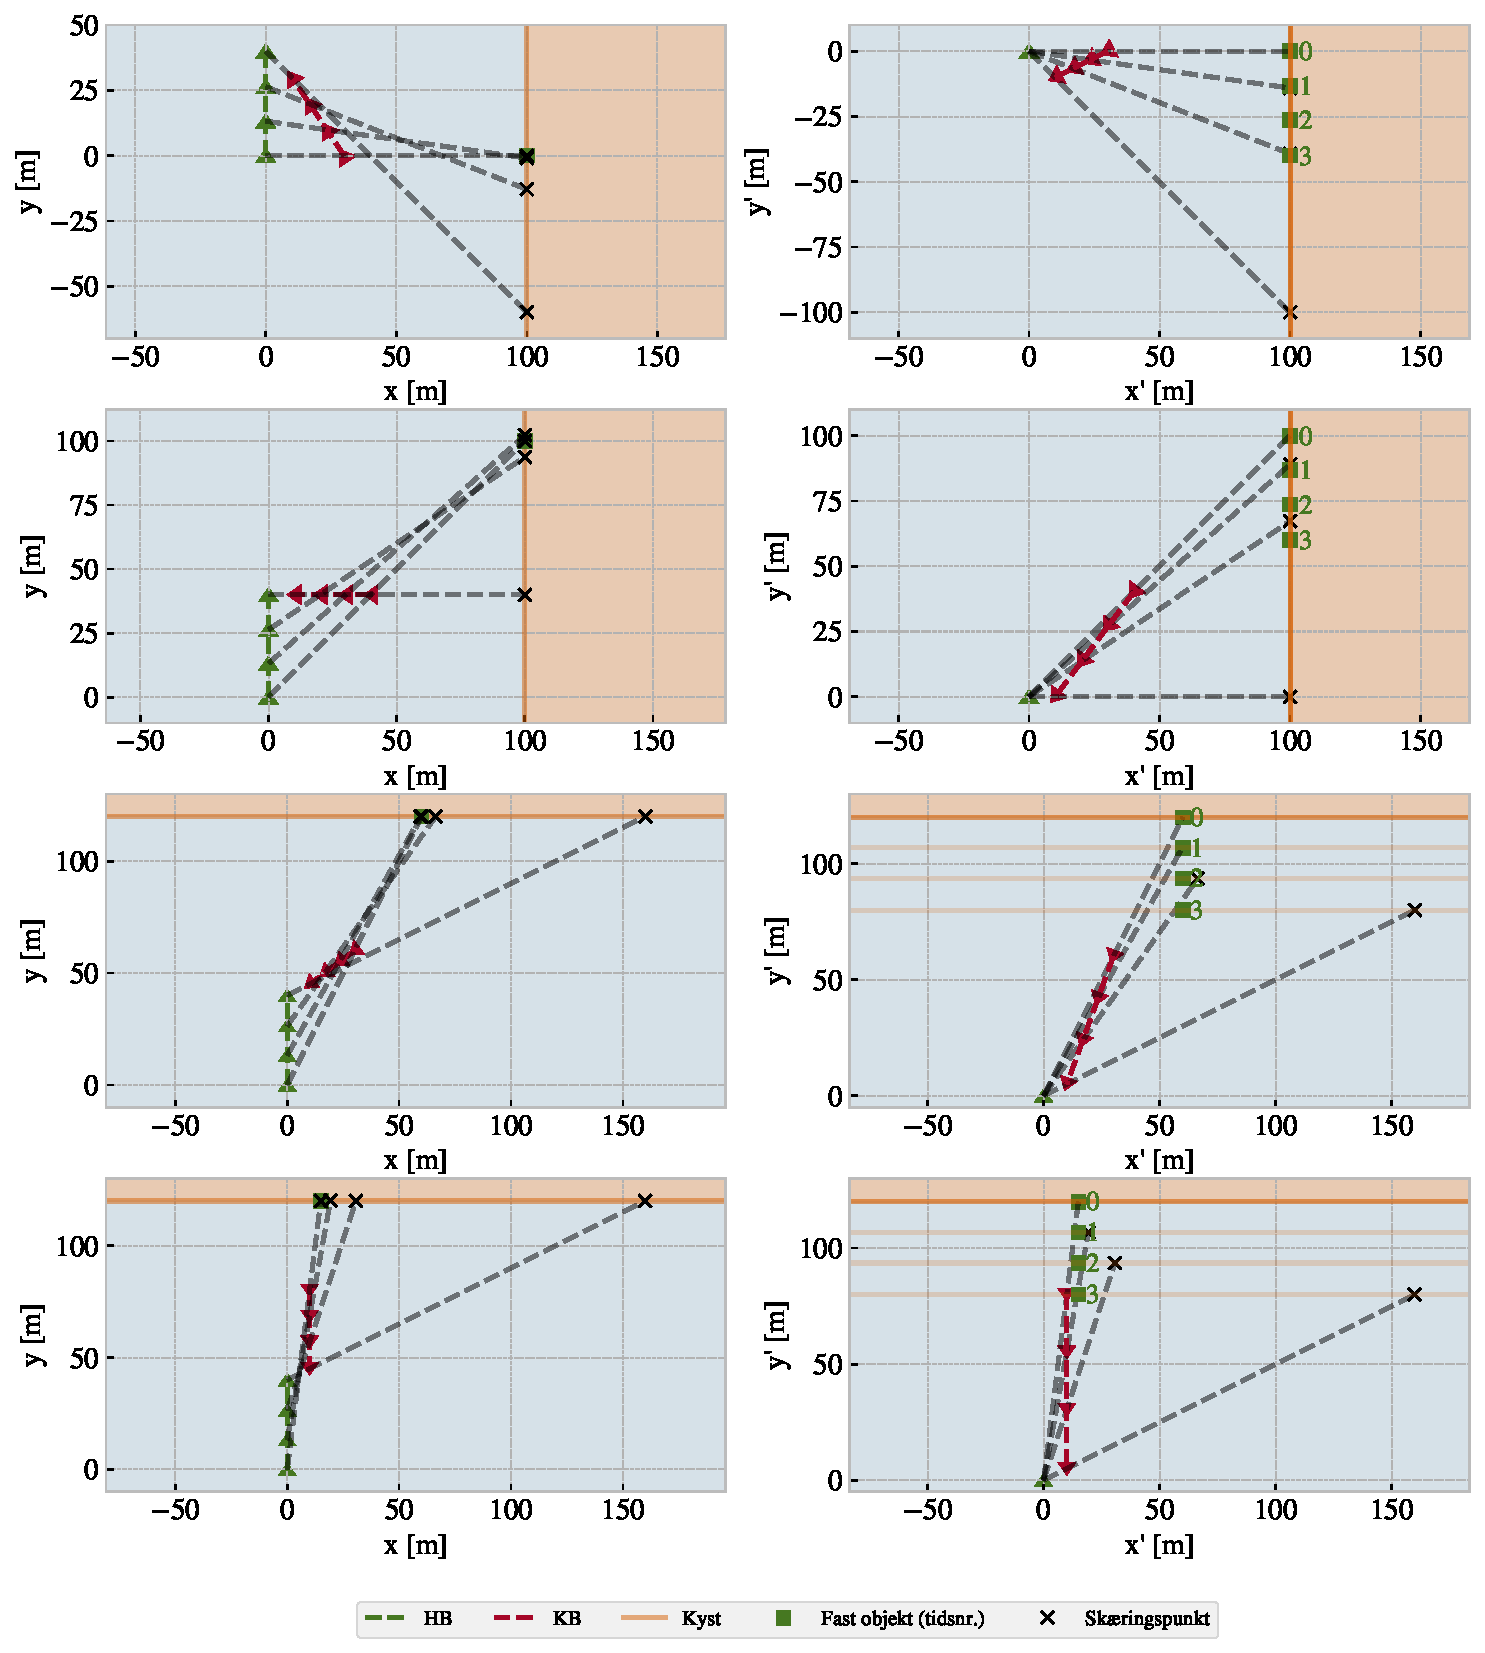
\includegraphics[width=\linewidth]{figures/subplot_NC1.pdf}
  \caption[A table inside a caption]{
\begin{tabular}{|c|c|c|c|c|}
\hline
Figurrække & $HB_{start}$  & $KB_{start}$ & $HB_{slut}$ & $KB_{slut}$\\ \hline
1  & (0,0) & (30,0) & (0, 40) & (10, 30) \\ \hline
2  & (0,0) & (40,40) & (0, 40) & (10, 40) \\ \hline
3  & (0,0) & (30,60) & (0, 40) & (10, 44) \\ \hline
4  & (0,0) & (10,80) & (0, 40) & (10, 44) \\ \hline
\end{tabular}}
  \label{fig:subplot_NC1}
\end{figure}








\end{document}
